\documentclass[./main.tex]{subfiles}

\begin{document}
\section{Deep Learning Theory}
The following section covers the most important background theory for the experiments in Section \ref{sec:experiments}. This includes an introduction to various types of neural networks, as well as an introduction to the optimization of such networks.

\subsection{Feedforward Neural Networks}
\textbf{Feedforward neural networks} are the most basic type of neural networks. The aim of a feedforward neural network is to approximate some function $f^*$, by defining a mapping $\bm{y} = f(\bm{x}; \bm{\theta})$ and learning the parameters $\bm{\theta}$, that results in the best approximation of $f^*$. These models are called \textbf{feedforward} because there are no \textbf{feedback} connections in which the outputs of the model are fed back into itself. Instead, information flows through the function being evaluated from $\bm{x}$, through the intermediate computations used to define $f$, and finally to the output $\bm{y}$. Feedforward neural networks generally consists of multiple \textbf{layers}, arranged in a chain structure, with each layer being a function of the layer that preceded it \cite{DL_book}. 

\subsubsection{Fully-connected Layers}
The most simple type of layer found in a feeforward neural network is the \textbf{fully-connected layer}. The fully-connected layer usually consists of some learnable parameter matrix and learnable parameter vector, as well as a \textbf{activation function}, which is a non-linear function, that makes it possible for the network to model non-linearity. Three of the most common activation functions are the \textbf{Rectified Linear Unit (ReLU)}, \textbf{Sigmoid} and \textbf{Hyperbolic Tangent (Tanh)} activation functions, defined as
\begin{align}
    &\text{ReLU}(x) = \max\{0, x\} \\ 
    &\text{Sigmoid}(x) = \sigma(x) = \frac{1}{1 + exp(x)} \\ 
    &\text{tanh}(x) = \frac{\exp(x) - \exp(-x)}{\exp(x) + \exp(-x)}
\end{align}
Given the learnable parameter matrix $\bm{W}$, learnable parameter vector $\bm{b}$ and activation function $g$, the $i$'th fully-connected layer is defined as
\begin{equation}
    \bm{h}^{(i)} =
    \begin{cases}
        g^{(i)} \left( \bm{W}^{(i) \top} \bm{h}^{(i - 1)} + \bm{b}^{(i)} \right) & \text{if } i > 1 \\
        g^{(1)} \left( \bm{W}^{(1) \top} \bm{x} + \bm{b}^{(1)} \right) & \text{if } i = 1
    \end{cases}
    .
\end{equation}
Thus, for a neural network with $n$ layers, we have the mapping \cite{DL_book}
\begin{equation}
    \bm{y} = f(\bm{x};\bm{\theta}) = \bm{h}^{(n)}.
\end{equation}

\subsubsection{Convolutional Layer}
\begin{figure}[htbp]
    \centering
    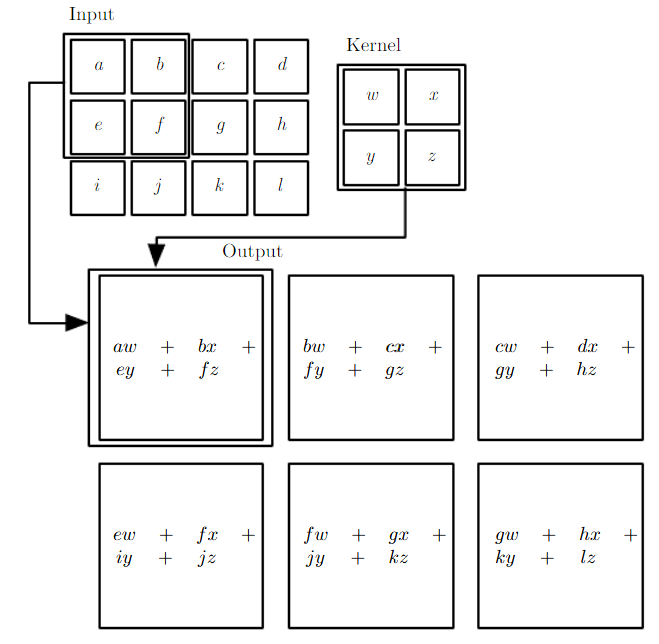
\includegraphics[width = 0.5 \textwidth]{./entities/2d_conv_example.PNG}
    \caption{An example of applying a 2d kernel on an input \cite{DL_book}.}
    \label{fig:2d_conv_example}
\end{figure}
\noindent A \textbf{convolutional layer} is a specialized kind of feedforward layer, usually used in analysis of time-series or image data. If a network has at least one convolutional layer, it is called a \textbf{Convolutional neural network (CNN)} \cite{DL_book}.
\\
\\
\noindent The convolutional layer consists of a set of \textbf{kernels}, each to be applied to the entire input vector, where each kernel is a learnable parameter matrix $k \times k$ \cite{everything}. Each kernel is applied on the input to produce a \textbf{feature map}. The kernels are applied to the input by "sliding" over the input (where the step size is called \textbf{stride}). Each $k \times k$ grid of the input is then used to compute the dot-product between the grid and each kernel, which is then placed in the corresponding feature map of each kernel, as visualized in Figure \ref{fig:2d_conv_example}. \cite{bsc_thesis}. To control the dimensions of the output, one might \textbf{pad} the sides with a constant value. Commonly, zero is used as the padding-value.
\\
\\
As seen in Figure \ref{fig:2d_conv_example}, each kernel produces a linear combination of all pixel values in a neighbourhood defined by the size of the kernel. Thus, unlike a fully-connected layer, a convolutional layer captures the high correlation between a pixel and its neighbours. Further, by limiting the size of the kernel, the network will use much fewer parameters, than if it was replaced by a fully-connected layer \cite{DL_book}.

\subsection{Recurrent Neural Networks}
\begin{figure}[htbp]
    \centering
    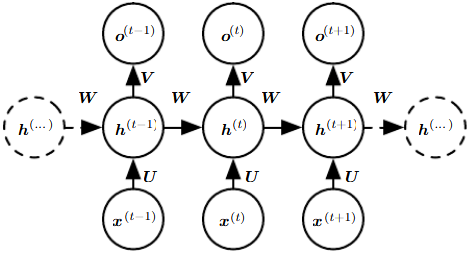
\includegraphics[width = 0.5 \textwidth]{./entities/rnn_illustration.PNG}
    \caption{An illustration of an RNN \cite{DL_book}.}
    \label{fig:rnn_illustration}
\end{figure}
\noindent \textbf{Recurrent neural networks (RNNs)} are a family of neural networks for processing sequential data. Figure \ref{fig:rnn_illustration} illustrates the general setup of such a network, which maps an input sequence of $\bm{x}$ values to a corresponding sequence of output $\bm{o}$ values. Generally, a RNN consists of three parts: (1) the input ($\bm{x}^{(i)}$), (2) the hidden state ($\bm{h}^{(i)}$), and (3) the output ($\bm{o}^{(i)}$). During inference, the model maps each input value to an output value in a sequential matter, where it first maps the first input value, then the second, then the third, and so forth. The network maps each input value to an output value by making use of the hidden state from the preceding step, where the first hidden state has to be initiallized \cite{DL_book}.

\subsubsection{Convolutional Long Short-Term Memory}
One common recurrent neural network unit is the \textbf{convolutional long short-term memory (ConvLSTM)}, which is an adaptation of the standard \textbf{long short-term memory (LSTM)} for sequences of images. Both LSTMs work by potentially stacking multiple \textbf{cells} together, such that each LSTM cell is taking in outputs of the preceding LSTM cell as its input. 
\\
\\
\noindent The idea of both LSTM cells is to create paths through time that have derivatives that neither vanish nor explode. This is done by introducing a memory cell $\mathsf{C}_t$, which accumulates state information over a long duration. This cell is accessed, written and cleared by several controlling gates. The model learns during training, when to access, write and clear this memory cell. By using the memory cell and gates to control the flow of information, the gradient will be trapped in the cell and thus be prevented from vanishing too quickly \cite{DL_book,conv_lstm}.
\\
\\
The ConvLSTM cell consists of three gates. The first gate is the input gate $\mathsf{I}_t$, which controls whether or not to accumulate the information of a new input to the cell. This gate is defined as
\begin{equation}
    \mathsf{I}_t = \sigma \left( \mathsf{W}_{xi} * \mathsf{X}_t + \mathsf{W}_{hi} * \mathsf{H}_{t - 1} + \mathsf{W}_{ci} \circ \mathsf{C}_{t - 1} + \mathsf{B}_i \right)
\end{equation}
where $\mathsf{X}_t$ is the current input image, $\mathsf{H}_{t - 1}$ is the hidden state of the previous time step, $\mathsf{C}_{t - 1}$ is the cell output of the previous time step, and $\mathsf{W}_{xi}$, $\mathsf{W}_{hi}$, $\mathsf{W}_{ci}$ and $\mathsf{B}_i$ are learnable parameters
\\
\\
The second gate is the \textbf{forget gate} unit $\mathsf{F}_t$ (at time step $t$), which controls whether or not to "forget" the status of the cell output of the previous time step. The forget gate is defined as
\begin{equation}
    \mathsf{F}_t = \sigma \left( \mathsf{W}_{xf} * \mathsf{X}_t + \mathsf{W}_{hf} * \mathsf{H}_{t - 1} + \mathsf{W}_{cf} \circ \mathsf{C}_{t - 1} + \mathsf{B}_f \right)
\end{equation}
where $\mathsf{W}_{xf}$, $\mathsf{W}_{hf}$, $\mathsf{W}_{cf}$ and $\mathsf{B}_f$ are learnable parameters.
\\
\\
The last gate is the \textbf{output gate} unit $\mathsf{O}_t$, which controls whether or not the latest cell output will be proagated to the final state $\mathsf{H}_t$. This cell is defined as
\begin{equation}
    \mathsf{O}_t = \sigma \left( \mathsf{W}_{xo} * \mathsf{X}_t + \mathsf{W}_{ho} * \mathsf{H}_{t - 1} + \mathsf{W}_{co} \circ \mathsf{C}_t + \mathsf{B}_o \right)
\end{equation}
where $\mathsf{W}_{xo}$, $\mathsf{W}_{ho}$, $\mathsf{W}_{co}$ and $\mathsf{B}_o$ are learnable parameters.
\\
\\
By combining the three gates, we get the following definition of the ConvLSTM Cell.
Let $\mathsf{X}_1, \mathsf{X}_2, ..., \mathsf{X}_t$ be a sequence of input images. Then, at each time step $t$, we compute
\begin{align}
    \mathsf{I}_t &= \sigma \left( \mathsf{W}_{xi} * \mathsf{X}_t + \mathsf{W}_{hi} * \mathsf{H}_{t - 1} + \mathsf{W}_{ci} \circ \mathsf{C}_{t - 1} + \mathsf{B}_i \right) \\
    \mathsf{F}_t &= \sigma \left( \mathsf{W}_{xf} * \mathsf{X}_t + \mathsf{W}_{hf} * \mathsf{H}_{t - 1} + \mathsf{W}_{cf} \circ \mathsf{C}_{t - 1} + \mathsf{B}_f \right) \\
    \mathsf{C}_t &= \mathsf{F}_t \circ \mathsf{C}_{t - 1} + \mathsf{I}_t \circ \text{tanh} \left( \mathsf{W}_{xc} * \mathsf{X}_t + \mathsf{W}_{hc} * \mathsf{H}_{t - 1} + \mathsf{B}_c \right) \\
    \mathsf{O}_t &= \sigma \left( \mathsf{W}_{xo} * \mathsf{X}_t + \mathsf{W}_{ho} * \mathsf{H}_{t - 1} + \mathsf{W}_{co} \circ \mathsf{C}_t + \mathsf{B}_o \right) \\
    \mathsf{H}_t &= \mathsf{O}_t \circ \text{tanh}(\mathsf{C}_t)
\end{align}
For $t = 1$, both $\mathsf{H}_{t - 1}$ and $\mathsf{C}_{t - 1}$ have to be initialized \cite{conv_lstm}.

\subsection{Transformer}
\begin{figure}[htbp]
    \centering
    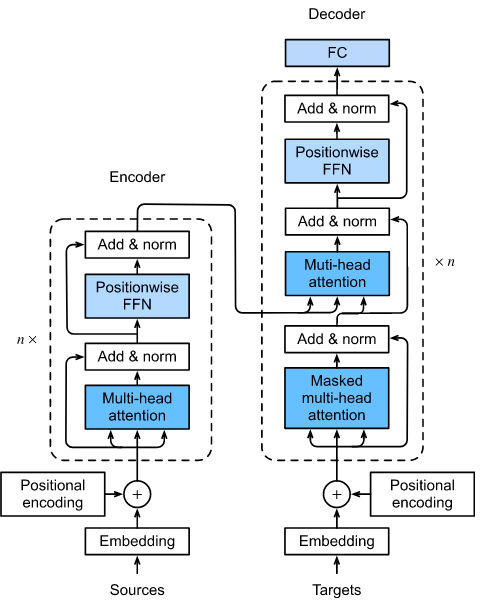
\includegraphics[width = 0.5 \textwidth]{./entities/transformer.PNG}
    \caption{An illustration of the Transformer architecture \cite{d2l}.}
    \label{fig:transformer_illustration}
\end{figure}
The sequential nature of RNNs precludes parallelization withing training examples, heavily slowing down the training of these models. Another type of model for sequential data is the \textbf{Transformer}, which eschews recurrence and instead relies on an \textbf{attention} mechanism to draw dependencies between input and output. The Transformer allows for more parallelization and can reach state of the art results \cite{https://doi.org/10.48550/arxiv.1706.03762}.

\subsubsection{Attention}
\begin{figure}[htbp]
    \centering
    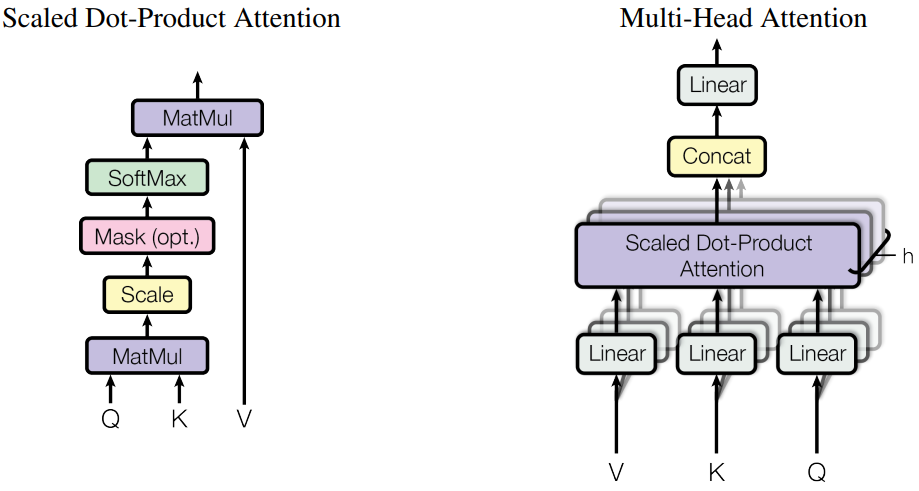
\includegraphics[width = 0.5 \textwidth]{./entities/attention.PNG}
    \caption{Illustration of (lef) the Scaled Dot-Product Attention, and (right) the Multi-Head Attention, which consists of several attention layers running in parallel \cite{https://doi.org/10.48550/arxiv.1706.03762}.}
    \label{fig:attention_illustration}
\end{figure}
\noindent An attention function is a function that maps a given query and a given set of key-value pairs to an output. In this function the query, keys, values, and output are all vectors, and the output is a weighted sum of the values, where the weight of each value if computed by a compatibility function of the query with the corresponding key \cite{https://doi.org/10.48550/arxiv.1706.03762}. Figure \ref{fig:attention_illustration} illustrates the two types of attention functions used in the Transformer.
\\
\\
\textbf{Scaled Dot-Product Attention:} The scaled dot-product attention is the core attention function of the transform. The function takes queries and keys of dimensions $d_k$ as input, and values of dimension $d_v$. In practice, the attention function is computed on a set of queries, keys and values simultaneously, by packing them into matrices $\bm{Q}, \bm{K}$, and $\bm{V}$, respectively. Thus, the scaled dot-product attention is computed as
\begin{equation}
    \text{Attention}(\bm{Q}, \bm{K}, \bm{V}) = \text{softmax}\left( \frac{\bm{Q}\bm{K}^T}{\sqrt{d_k}} \right) \bm{V}
\end{equation} 
where the scaling of $\bm{Q}\bm{K}^T$ is done to counteract the cases with a large $d_k$, which would result in the softmax-function having an extremely small gradient \cite{https://doi.org/10.48550/arxiv.1706.03762}.
\\
\\
\textbf{Multi-Head Attention:} The \textbf{multi-head attention} is the used attention function by the Transformer and is an extention to the scaled dot-product attention. This attention function linearly projects the queries, keys and values $h$ times with different, learned linear projections to $d_k$, $d_k$, and $d_v$ dimensions, respectively. For each of the projected queries, keys and values, the scaled dot-product attention is applied, yielding $d_v$-dimensional output values. These output values are finally concatenated and further projected, resulting in the final values. By using multi-head attention, the model is allowed to jointly attend to information from different representation subspaces at different positions \cite{https://doi.org/10.48550/arxiv.1706.03762}.

\subsubsection{The Architecture}
The Transformer follow an encoder-decoder structure, where the encoder maps an input sequence $\bm{x}$ to a sequence of continuous representations $\bm{z}$. The decoder then uses $\bm{z}$ to generate an output sequence $\bm{y}$, one element at a time. At each step the model consumes the previously generated output element as additional input when generating the next output \cite{https://doi.org/10.48550/arxiv.1706.03762}. Figure \ref{fig:transformer_illustration} illustrates the overall architecture of the Transformer.
\\
\\
\noindent \textbf{Encoder:} The encoder consists of $N$ identical layers, where each layer consists of two sub-layers. The first sub-layer is a multi-head \textbf{self-attention} layer, and the second sub-layer is a position-wise fully-connected feedforward network. Around each sub-layer is a \textbf{residual connection}, where the the input of the sub-layer is added to the output of the sub-layer. This residual connection is then followed by a round of \textbf{layer normalization}. In this self-attention layer the keys, values and queries come from the output of the previous layer in the encoder. Each position in the encoder can attend to all positions in the previous layer of the encoder \cite{https://doi.org/10.48550/arxiv.1706.03762}.
\\
\\
\noindent \textbf{Decoder:} The decoder also consists of $N$ identical layers. In addition to the two sub-layers in each encoder layer, the decoder also consists of a third sub-layer, which performs multi-head attention over the output of the encoder stack (called \textbf{cross-attention} \cite{cross_attention}). Also here, is residual connections used around each of the sub-layers, followed by layer normalization. To ensure, that the predicitons for position $i$ only depends on the known outputs at positions less than $i$, the self-attention sub-layer in the decoder stack is modified. This self-attention sub-layer, allows each position in the decoder to attend to all positions in the decoder up to and including that position. The self-attention sub-layer is modified by masking out all values in the input of the softmax which correspond to illegal connections \cite{https://doi.org/10.48550/arxiv.1706.03762}.
\\
\\
\noindent \textbf{Feedforward Networks:} Each of the layers in the encoder and decoder contains a fully-connected feedforward layer, consisting of two linear transformations with the ReLU activation-function applied in between, as described below \cite{https://doi.org/10.48550/arxiv.1706.03762}
\begin{equation}
    FFN(\bm{x}) = \max \left(0, \bm{x} \bm{W}_1 + \bm{b}_1 \right) \bm{W}_2 + \bm{b}_2.
\end{equation}
\\
\\
\noindent \textbf{Positional Encoding:} As the model does not contain any recurrences nor any convolutions, it has to carry some other type of information to know about the relative or absolute position of the elements in the input sequence. This is done by adding \textbf{positional encodings} to the input of the encoder and decoder stacks. The positional encoding is a vector of size $d_{model}$ and is defined as the following
\begin{align}
    \bm{PE}_{pos, 2i} &= \sin \left( \frac{pos}{10000^{\frac{2i}{d_{model}}}} \right) \\
    \bm{PE}_{pos, 2i + 1} &= \cos \left( \frac{pos}{10000^{\frac{2i}{d_{model}}}} \right) \\
\end{align}
where \textit{pos} is the position and $i$ is the dimension \cite{https://doi.org/10.48550/arxiv.1706.03762}.

\subsection{General Machine Learning Terminology}
The following section covers the general terminology and some algorithms, that will be used through this paper. 
\\
\\
\noindent \textbf{Loss Function:} Training a machine learning model is generally done by minimizing a predefined \textbf{loss function}, which is used for measuring the error of the model. One common loss function for regression is the \textbf{Mean Squared error (MSE)}. Let $f^*(\bm{x})$ be a vector of ground truth observations and $f(\bm{x}; \bm{\theta})$ be an estimation of $f^*(\bm{x})$. Then, MSE is defined as
\begin{equation}
    MSE = \frac{1}{n} \sum_{i = 1} ^n \left( f^*\left(\bm{x}^{(i)}\right) - f\left(\bm{x}^{(i)}; \bm{\theta}\right)\right)^2.
\end{equation}
Thus, MSE measures the average squared difference between the ground truth observations and the estimated observations \cite{ISL}.
\\
\\
\noindent \textbf{Optimizer:} The minimization of the loss function is usually done by an \textbf{optimizer}, which is a type of algorithm, that is typically some type of variation of \textbf{gradient descent}. Gradient descent is a process that iteratively updates the parameters of a function by
\begin{equation}
    \bm{\theta} \leftarrow \bm{\theta} - \eta \nabla_{\bm{\theta}} L\left( f\left(\bm{x}^{(i)}; \bm{\theta}\right), f^*\left(\bm{x}^{(i)}\right) \right)
\end{equation}
where $\eta$ is called the \textbf{learning-rate}, which controls the stepsize of each update, and $L$ is a loss function such as MSE.
\\
\\
One of the most used optimizers is \textbf{ADAM}, which is an optimizer that uses \textbf{momentum} and \textbf{adaptive learning-rate} to accelerate its learning. Momentum works by accumulating an exponentially decaying moving average of past gradients and continuing to move in their direction, which especially accelerates learning in the face of high curvature, small but consistent gradients, or noisy gradients. Adaptive learning rate is a mechanism for adapting individual learning rates for the model parameters. The idea is as follows; if the partial derivative of the loss, with respect to a given model parameter, remains the same sign, then the learning rate should increase. If that partial derivate changes sign, then the learning rate should decrease. The algorithm uses a hyperparameter $\rho$ for controling the length scale of the moving average The pseudocode of the algorithm has been illustrated in Algorithm \ref{Algorithm:ADAM}. \cite{DL_book}. 
\\
\\
\noindent \textbf{Online, mini-batch and batch gradient methods:} Unlike gradient descent, ADAM bases its computations on a \textbf{mini-batch} of samples instead of basing it on a single sample. Thus, there are three ways of sampling data for the optimizer. The first way is done by sampling a single sample at each iteration. This class of methods is called \textbf{online gradient methods}. The advantage of these methods is, that each iteration is very quick, as we only have to compute the gradient of a single sample, however, the main disadvantage is, that the algorithm uses a lot of iterations. On the other hand we have \textbf{batch gradient methods} which uses the average gradient of all of the $n$ samples of the dataset to comptute $\nabla L(f(\bm{x}, \bm{y}))$. By doing so the algorithm only requires one iteration, however, this iteration is much slower than each iteration of the online gradient methods. The last class of methods is \textbf{mini-batch gradient methods} which uses the average gradient of $|B|$ samples of the dataset for computing $\nabla L(f(\bm{x}, \bm{y}))$, where $B$ is a predefined hyperparameter called the \textbf{mini-batch size}. This method lies in between the online gradient methods and batch gradient methods, as it uses fewer iterations than the online gradient methods, however, it uses more iterations than the batch gradient methods. Likewise, each iteration is faster to compute than it is for the batch gradient methods, but slower than it is for the online gradient methods. Further, online gradient methods can lead to a very noisy learning process due to the high variance of the computed gradients of the samples, which can make it more difficult for the optimizer to reach the minimum of the loss function. mini-batch gradient methods and batch gradient methods removes this noise by averaging the computed gradient at each iteration, essentially leading to a quicker learning process \cite{DL_book}. 
\\
\\
\begin{algorithm}[htbp]
    \caption{Adam \cite{DL_book}}
    \label{Algorithm:ADAM}
    \begin{algorithmic}
        \Require Learning rate $\eta$
        \Require Exponential decay rates for moment estimates, $\rho_1$ and $\rho_2$ in $[0, 1)$
        \Require Small constant $\delta$ used for numerical stabilization
        \Require Initial parameters $\bm{\theta}$
        \State Initialize 1st and 2nd moment variables $\bm{s} = \bm{0}$, $\bm{r} = \bm{0}$
        \While{stopping criterion not met}

            \State \begin{varwidth}[t]{\linewidth} Sample a minibatch of $m$ random observations from the training set $\{\bm{x}^{(1)}, ..., \bm{x}^{(m)}\}$ with corresponding targets $\bm{y}^{(i)}$
            \end{varwidth}
            \State Compute gradient: $\bm{g}  \leftarrow  \frac{1}{m} \nabla_{\bm{\theta}} \sum_i L\left( f \left(\bm{x}^{(i)}; \bm{\theta} \right), \bm{y}^{(i)} \right)$
            \State $t \leftarrow t + 1$
            \State Update biased first moment estimate: $\bm{s} \leftarrow \rho_1 \bm{s} + (1 - \rho_1) \bm{g}$
            \State Update biased second moment estimate: $\bm{r} \leftarrow \rho_2 \bm{r} + (1 - \rho_2) \bm{g} \odot \bm{g}$
            \State Correct bias in first moment: $\hat{\bm{s}} \leftarrow \frac{\bm{s}}{1 - \rho_1 ^t}$
            \State Correct bias in second moment: $\hat{\bm{r}} \leftarrow \frac{\bm{r}}{1 - \rho_2 ^t}$
            \State Compute update: $\Delta \bm{\theta} = - \eta \frac{\hat{\bm{s}}}{\sqrt{\hat{\bm{r}}} + \delta}$
            \State Apply update: $\bm{\theta} = \bm{\theta} + \Delta \bm{\theta}$ 
        \EndWhile
    \end{algorithmic}
\end{algorithm}

\noindent \textbf{Layer Normalization: } One problem when optimizing a neural network is, that the gradients with respect to the weights of one layer depends on the outputs of the neurons of the previous previous layer. If these outputs change in a highly correlated way, the model could experience some undesired "covariate shift", which would make the training take longer. One way to reduce these "covariate shifts" is to make use of \textbf{layer normalization}, where the layer normalization statistics over all the hidden units in the same layer $l$ is computed as the following
\begin{equation}
    \mu^{(l)} = \frac{1}{H} \sum_{i = 1} ^H \bm{w}_i^{(l)^\top}\bm{h}^{(l - 1)}, \quad \sigma^{(l)} = \sqrt{\frac{1}{H} \sum_{i = 1} ^H \left(\bm{w}_i^{(l)^\top}\bm{h}^{(l - 1)} - \mu^{(l)}\right)^2}
\end{equation}
where $H$ is the amount of hidden units of the $l$th layer, $\bm{w}_i^{(l)}$ is the incoming learnable weight vector to the $i$th hidden unit of the $l$th layer, and $\bm{h}^{(l - 1)}$ is the output of the preceding layer. Thus, the summed inputs $\bm{w}^{(l)^\top} _i \bm{h}^{(l - 1)}$ is normalized and rescaled by
\begin{equation}
    \bar{a}_i = \frac{\bm{w}^{(l)^\top} _i \bm{h}^{(l - 1)} - \mu^{(l)}}{\sigma^{(l)}}.
\end{equation}
Further, the input to the current layer $l$ also learns an adaptive bias $b$ and gain $g$ for each neuron after the normalization. Thus, the $i$th input to layer $l$ is defined as the following
\begin{equation}
    h_i ^{(l)} = f\left(\frac{g_i(a_i - \mu^{(l)}) + b_i}{\sigma^{(l)}} \right)
\end{equation}
where $f$ is a non-linear activation function \cite{ba2016layer}.

\noindent \textbf{Evaluation:} We often want to know how well a machine learning model performs on an unseen sample. This is commonly done by splitting the dataset into three non-overlapping subsets to avoid a biased evaluation. The first dataset is the \textbf{training} dataset which is used for training the machine learning model. The second dataset is the \textbf{validation} dataset which is used during training for evaluating various settings of the the used (hyper)parameters. The last dataset is the \textbf{testing} dataset, which is then used for evaluating the final machine learning model.
\\
\\
The evaluation of a machine learning model is done by making use of an \textbf{evaluation metric}, which depends on the task of the machine learning model. For pose estimation, the \textbf{Percentage of Correct Keypoints (PCK)} is commonly used. This metric measures the ratio of predicted keypoints that are closer to their corresponding ground-truth keypoints than some threshold. Often \textbf{PCK@0.2} is used, which uses $20\%$ of the torso diameter as its threshold \cite{https://doi.org/10.48550/arxiv.2001.08095}.
\\
\\
\noindent \textbf{Dropout:} A machine learning model is said to be \textbf{overfitting} if the loss of the training dataset is decreasing, while the loss of the validation dataset is increasing. One can make use of a group of technies called \textbf{regularization} to avoid the overfitting of the network. One common regularization technique is \textbf{dropout}, where the each parameter of the machine learning model is randomly disabled with probability $p$ during training. By doing so the parameters are being trained on the dataset fewer times, leading to less of a probability of the model overfitting.
\\
\\
\noindent \textbf{Epoch:} Often, the optimizer needs multiple "rounds" of using the whole training data for reaching its minimum. Each of these rounds is called an \textbf{epoch}. One can pick the number of epochs to iterate through prior to training a model and just stop the training once the optimizer has used all of its epochs. Another methods is to use \textbf{early-stopping}, where one keeps track of the loss of the model on the validation-set for each epoch. Once the validation-loss has not decreased for $n$ consecutive epochs, the training is terminated.

\end{document}